\documentclass[12pt] {article}

\usepackage[margin=1in]{geometry} %one inch margins
\renewcommand{\baselinestretch}{2} %double space, safe for fancy headers
\usepackage{pslatex} %Times font
\usepackage{apacite} %apa citation style
\bibliographystyle{apacite}
%\usepackage[pdfborder={0 0 0}]{hyperref}%for hyperlinks without ugly boxes
\usepackage{graphicx} %for figures
\usepackage{enumerate} %for lists
\usepackage{fancyhdr} %header
\pagestyle{fancy}
\usepackage[font={small,sf},format=plain,labelfont=bf,up]{caption}
\usepackage{indentfirst}

\fancyhf{}
\fancyhead[l,lo]{Qiao Zhang \textit{ CSE8317 Project Report}} %left top header
\fancyhead[r,ro]{\thepage} %right top header

\begin{document}
\title{Building a Knowledge Graph from Historical Defect Reports with Orthogonal Defect Classification}
\author{Qiao Zhang}
\date \today
\maketitle

\thispagestyle{empty}

\bigskip
%\tableofcontents
\pagebreak
\setcounter{page}{1}
\section{Introduction}
I'm making a change here

Defect report is commonly a structured natural language artifact generated during the software reliability engineering process.
A well-structured defect report would be very informative to viewers and very efficient for knowledge acquisition purpose.
The previous experience (or knowledge) of handling a specific type of defect would be critical to the success of the future defect analysis and process.
However, retrieving knowledge from the historical defect reports could be a painful job especially when the volume of reports is high enough.
Based on the experience of a well-known telecommunication equipment company, the number of their historical defect reports has reached 3 million and the number of newly generated defect reports is about 30 thousand each month.
Without an appropriate approach to standardize, formalize, and organize the historical defect reports, it is nearly impossible to retrieve knowledge from the gigantic pool of reports.\par

Ontology, as a formal and explicit specification of a shared conceptualization with a complex semantic web structure, is able to standardize and formalize a domain knowledge or the expert interpretation \cite{christina2016an}.
With orthogonal defect classification (ODC), we can not only classify the defect reports into a few specific types but also fit newly generated defect reports into some pre-determined workflows to improve the engineering efficiency.
Both approaches are able to contribute the the objective of improving the knowledge acquisition tasks in software reliability engineering regarding defect handling. 
It might be more beneficial to have them combined as one mechanism since one plus one can be more than two.
Knowledge Graph (KG), which integrates information from various types of resources into an ontology and also applies a reasoning engine to assist deriving new knowledge \cite{ehrlinger2016towards}, is promising to integrate the ODC results into the ontology to effectively and efficiently achieve certain types of knowledge acquisition tasks.
This project aims at conducting a feasibility study to explore the methodoly to manually build a KG from historical defect reports with ODC.

\section{Background}
\subsection{Ontology}
By formally defining the relationships among entities, ontology is able to provides the intuition of how to further derive the domain knowledge.
As a concept-level knowledge representative for sharing purpose, the potential benefits of applying ontology includes \cite{christina2016an}:
\begin{itemize}
    \item Provide explicit and consistent views of knowledge and distributed information
    \item Support communication among entire software engineering team 
    \item Enable automated data processing and analysis
    \item Improve search quality by taking advantage of its semantic web structure
\end{itemize}
\shortciteA{iliev2012automated} have investigated using ontologies to automatically predict the defect severity based on designed knowledge.
However, it is already beyond the scope of ontology since the author has already introducted a reasoning engine to derieve new knowledge.  
In other word, the ontology might be insufficient for defect analysis especially for an specific instance-level analysis task. 

\subsection{Knowledge Graph}
Knowledge Graph (KG) research has been concentrated by the state-of-the-art literature in recent years since Google posted a blog entry and described how they use KG to enhance their search engine in 2012\footnote{https://googleblog.blogspot.co.at/2012/05/introducing-knowledge-graph-things-not.html}.
The definition of KG has been various from each other until \shortciteA{ehrlinger2016towards} conducted a literature review to synthesize all definitions.
Based on the literature review results, the KG consists of knowledge base and reasoning engine while the ontology is one specific type of knowledge base.
Thus, the defect severity analysis methodology from \shortciteA{iliev2012automated} is very close to the definition of KG, and it proves the necessity of applying KG to the defect analysis domain. 
However, the KG has larger scope than ontology since it is able to integrate more information from different resources as an instance-level knowledge representative. 

\subsection{Orthogonal Defect Classification}
Orthogonal defect classification (ODC) has been known to reduce the effort of defect analysis especially for root cause analysis \cite{buglione2006introducing}.
With identified root cause, the classified defects can be put into pre-determined workflows that are carefully designed for processing defect effectively and effciently. 
Most existing defect classification approaches and processes are ad hoc and significantly relied on the experience of historical projects and domain expert knowledge of analysts. 
Once the amount of un-classified defects has been accumulated to a certain amount, it will become impossible to be conducted for the ODC analysis.
\shortciteA{huang2015autoodc} have proposed a learning-based automatic ODC (AutoODC) approaches by casting it as a supervised text classification problem.
In this study, the proposed KG is trying to integrate the ontology which contains syntatic data retrieved from defect reports, with the ODC results which can be either manually evaluated or automatically derieved with AutoODC.  

\section{Methodology}
\subsection{Data Collection}
The defect reports investigated in this research are provided by a large telecommunication equipment company with sensitive data desensitized.
The size of dataset to be observed is 10,000 defect reports and most defect reports are bilingual which increased the difficulty of applying AutoODC.
Since the application of AuotODC is not the concentration of this study, we can assume that the ODC analysis can be successfully conducted while the ODC results used in this study are actually derieved manually.
However, the AutoODC is a critical component to the success of building a KG of defect handling since the actual volumn of historical defect reports of the company is considerablely huge.
Due to the privacy consideration and disclosure policy, it is not possible for us to collect the details of how the company process the defect once it is reported and categorized.
The defect handling process mentioned in this study are mostly interpreted from the ``solution" part of defect reports and simulated based on the existing knowledge.

\subsection{Building Knowledge Graph}
According to the definition provided by \shortciteA{ehrlinger2016towards}, the design of KG consists of (1) the generation of ontology and (2) the development of reasoning engine.
\subsubsection{Generate Ontology}\label{sec:generate}
Manually building an ontology is commonly an incremental process.
The ontolgy starts with an initial node ``defect report" which is a kind of artifact generated in the software process.
By observing the existing elements included in defect reports, we are able to find the common attributes of them while each attribute will be a new node connected to the initial node.
Some nodes can be further extended into a set of sub-nodes if a detailed analysis is necessary or the sub-nodes have relationships with other nodes in the ontology.  
For instance, the description is a node connected to the defect report while the code snippet in the description can be a sub-node linked to a specific test case (in the testing knowledge domain) or a class-level file in the repository (in the development knowledge domain).
By repeating above extension work, the initial ontology of defect reports will be generated and waiting to be expanded by finding the external relationships that links the ontology to other knowledge domain.
In this study, the possible external knowledge domain other than the defect report ontology includes defect analysis, code development, testing, risk management, human resource and so on.  
Because the ontology generated in this study aims at the knowledge acquisition task of handling defect reports, we only need to consider the nodes (e.g., artifacts, activities, analysis results, etc.) that are closely related to the defect report handling process.
Once the entire ontology is generated manually, it can be further expaned with some automatic methodologies, however, it is not in the scope of our discussion.
\subsubsection{Develope Reasoning Engine}
The reasoning engine is designed and developed based on the possible knowledge acquisition tasks involved in the KG.
In this study, the objective is to build an KG that improves the effectiveness and efficiency of knowledge acquisition during the process of handling a defect report once the ODC result retrieved.
Hence, the reasoning flow of the reasoning engine should always start from a node in the defect report ontology or a node which represents a category of the ODC results.
For instance, a software realibility engineer might found the description of replication steps familiar; he or she would like to find a similar historical defect report; instead of searching a defect report with a keyword-based search engine, the KG would be able to retrieve a list of reports by using different reasoning flow, such as ``replication step of defect report A --- defect report A --- reported by P --- defect report B".
This will be discussed in the section \ref{sec:reasoning}.

\section{Results and Discussion}
\subsection{Ontology}
This section describe the incremental process of manually generating the ontology that will be upscaled to KG.
The generation is based on the objective of simulating the methodology of building a KG from historical defect reports with ODC results.
Hence, as a feasibility study, the generated ontology (or KG) is only a partial of the applicable KG version.
\subsubsection{Ontology of defect report}
\begin{figure*}[h]
    \centering
    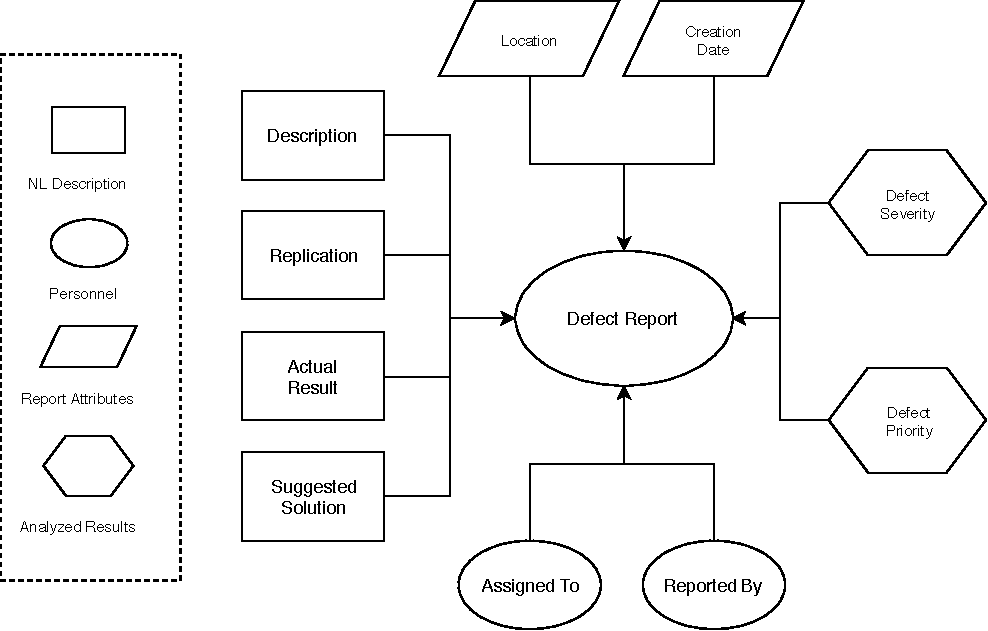
\includegraphics[width=0.8\textwidth]{../figures/OntologyOfDefectReport.pdf}
    \caption{Ontology generated based on defect report}
    \label{fig:defectreport}
\end{figure*}
The figure \ref{fig:defectreport} shows the nodes included in the defect report ontology before a further extension.
The square shape nodes represents all natural language contents included in the defect report while all natural language description can be further processed and characterized with natural language processing (NLP) technology.
For instance, the suggested solutions of all defect reports can be vectorized by words after pre-processing; the analysis on the vectorized matrix could provide useful knowledge to summarize the common solutions and create a set of new nodes in the KG; these nodes can be further connected to the defect reports based on its characteristics. 
Furthermore, the natural language contents of defect reports can be leveraged by AutoODC approached for defect classification.
In our KG, the ODC result of each defect report is essential to the reasoning mechanism of the reasoning engine regarding the knowledge acquisition tasks.
Each defect report can be considered as a layer of instance-level ontology while the connections between layers are critical to the propogation of reasoning flow among the KG. 
The ODC results could generate a considerable amount of connections between defect reports since every defect should have a category.
Hence, the square shape nodes will be extended to the ODC knowledge domain and in charge of bridging defects as well as defect reports.\par

The ellipse shape nodes represents all personnel information that should be linked to an external knowledge domain --- human resource.
The personnel information could help us find important reasoning flow, such as a certain type of defect can be easily found in a specific development or testing team.
However, this kind of information can be easily overlook in the defect analysis.
The haxagon shape nodes represents the attributes that can only be derieved by certain anlysis, such as defect severity, defect priority, and so on.
Because the KG is able to integrate more inforamtion from different resource, the results of all kinds of analysis are also important to the reasoning activity in KG.
However, not all analysis results should be included in the KG.
That is the reason why we always need to remember the objective of building the KG.
And finally, the parallelogram shape nodes represents the basic attributes of a defect report such as product name, release date, release version, and so on.
\subsubsection{Ontology with external knowlege domain}
The figure \ref{fig:external} demonstrates how defect report ontology and ODC categories could interact with ontologies of other knowledge domain.
This figure actually describes the process of handling a defect or a defect report on the concept-level and from the software process point of view.
A defect report will be conducted an ODC analysis and assigned an ODC category.
Based on the ODC category, the software reliability engineer will decide if it is possible and necessary to replicate the defect.
If so, the classified defect will be handed out to the testing team where a possible solution might be suggested.
On the other hand, the ODC category will provide candidate methodologies and specified knowledge domain information to assist the human resource (HR) ontology to find an appropriate analyst to conduct the defect analysis.
Once the defect has been analyzed (e.g., defect severity, defect priority, etc.), it is necessary to have a risk management team to evaluate the risk level which will be used to determine the further development plan.
If it is the time to fix the defect, the updated defect report will be able to provide guidance and accelerate the refactoring process.\par
\begin{figure*}[h]
    \centering
    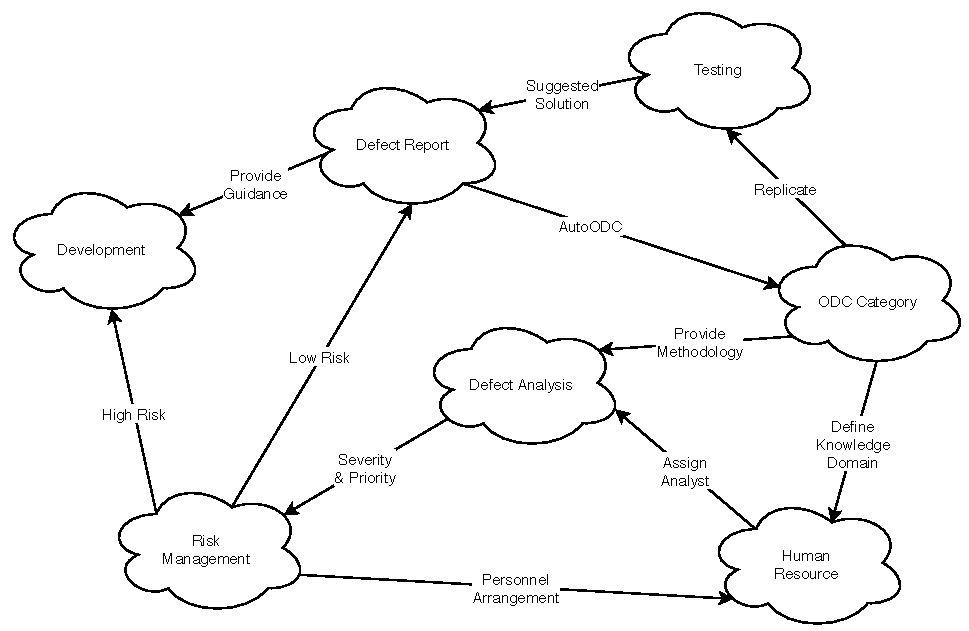
\includegraphics[width=0.8\textwidth]{../figures/OntologyOfExternal.pdf}
    \caption{Ontology with ODC and other external knowledge domain}
    \label{fig:external}
\end{figure*}
Due to the limited time and resource, the figure \ref{fig:external} is not detailed enough to show the connections between different knowledge domain in a node or sub-node level.
However, it is critical to have the ontologies designed as thorough as possible so that it can be upscaled to KG.
The major difference between ontology and KG is that the KG is an instance-level knowledge representative which integrates much more information than the ontology.
For instance, in the ontology, all the defect analysts will be considered as a single node in the HR ontology while every analyst should be a node in the KG. 
Different analyst may have different experience of the historical defect handling.
That is also the reason why we need use KG to achieve a specific instance-level knowledge acquisition task.

\subsection{Knowledge Graph and Reasoning Engine}\label{sec:reasoning}
One significant difference between ontology and KG is that the KG is apparently a 3-dimensional organization than a 2-dimentional representative (as shown in figure \ref{fig:kg}).
From the defect report point of view, each report can be an initial node (as discussed in section \ref{sec:generate}) and further expanded into a layer of instance-level ontology. 
With a group of defect reports, the multi-layer organization makes the KG a 3D strcuture.
Because there are links between layers, the KG is able to reasoning from layer to layer, as known as from instance to instance.
If the objective of the knowledge acquisition task is to start from a specific node (e.g., artifact, natural language description, etc.) and end up with another specific node (e.g., historical artifact, knowledge, fact, etcs.), the KG would be able to provide a huge number of condidate reasoning flow.
This subsetion will introduce the powerfulness of KG by using example.
\subsubsection{Defect Report to Defect Report}
Assuming the acquisition task is proposed by an analyst, the objective is to find a defect report (DR) that can provide intuition of processing the current DR as the DR-A in the figure \ref{fig:kg}.
There are several reasoning flows that can lead us from DR-A to the target node DR-B.
First of all, both DR-A and DR-B report that the defect is located in module-M; we can filter out a set of historical defect reports based on the location of defect with reasoning flow DR-A --- Location --- DR-B. 
However, it might not be a wise choice since the size of filtered reports could be still very high, and that is the reason why we need more than one reasoning flow.
From the testing and refactorign perspective, DR-A and DR-B have different replication steps but they have the same testing suite and refactoring solution because both defect caused by a critical step --- Step-A.
Comparing the filtered results based on the location of defect, we will be able to have a more precise list of defect reports that should contain the DR-B which is the ground truth.
\subsubsection{Solution to R}


\begin{figure*}[h]
    \centering
    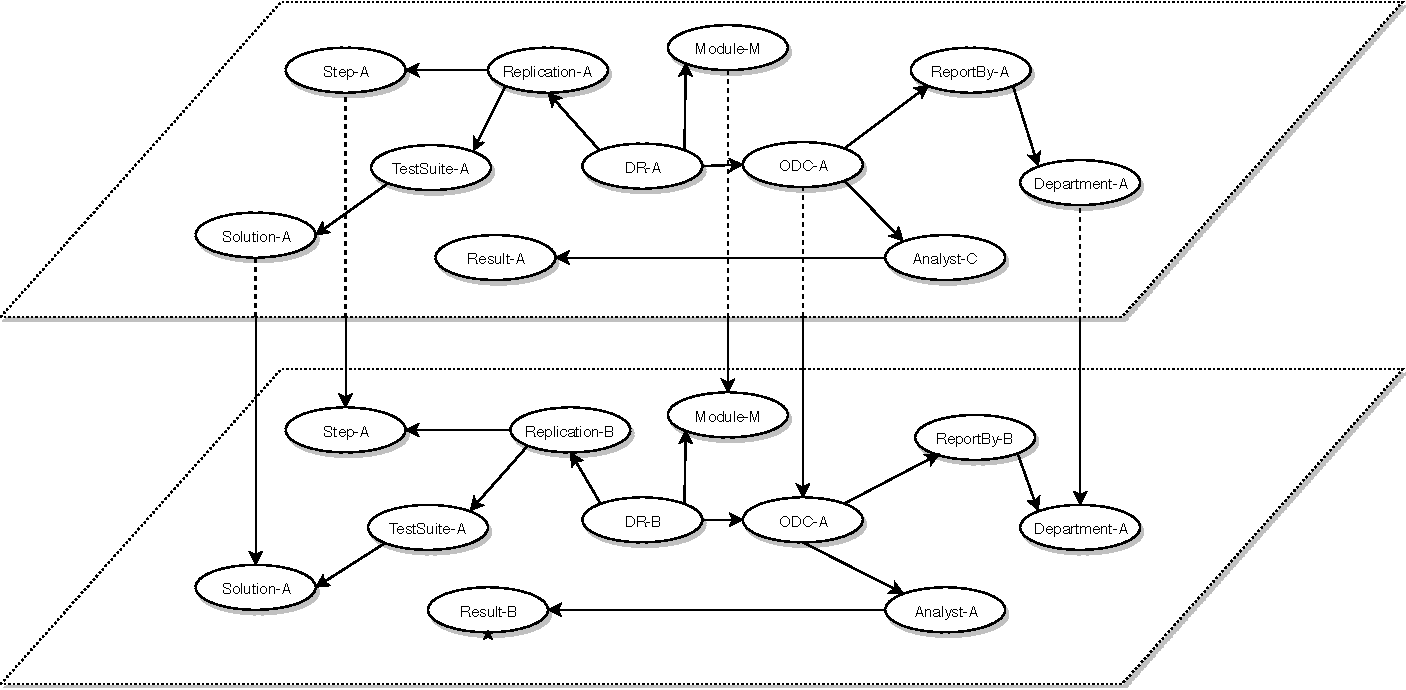
\includegraphics[width=0.95\textwidth]{../figures/KnowledgeGraph.pdf}
    \caption{Demonstration of instance-level knowledge graph and reasoning engin}
    \label{fig:kg}
\end{figure*}
\subsection{Application Scenario}

\section{Conclusion and Future Works}


\pagebreak
\bibliography{../bib}{project} %rename to your .bib file
\end{document}
